%%
% BIThesis 本科毕业设计论文模板 —— 使用 XeLaTeX 编译 The BIThesis Template for Undergraduate Thesis
% This file has no copyright assigned and is placed in the Public Domain.
%%

% 第一章节
\chapter{系统模块的设计}

\section{总体设计}

\textcolor{black}{本文涉及了一种基于强化学习Sarsa算法的静态对抗性样本生成系统,主要包含如下的几个模块:样本筛选模块,恶意程序扫描模块,强化学习静态对抗性样本生成模块。}

\textcolor{black}{其中,样本筛选模块的功能是,对于VirusShare网站上收集到的样本,其后缀名加上.exe,因为下载VirusShare原始样本时,该网站为了避免危害用户计算机,会默认去除恶意软件的后缀名。对于国内反病毒软件论坛上收集到的样本,需要去除非exe后缀的文件或文件大小较大的文件。强化学习对抗性样本生成模块只允许输入经由样本筛选模块后得到的筛选后样本。恶意程序扫描模块的功能是,使用ClamAV对收集到的原始恶意样本进行扫描,得到原始恶意样本检出率,以及对处理后的恶意样本进行扫描,得到处理后恶意样本检出率,以及供强化学习对抗性样本生成模块判定处理后的样本能否逃逸静态检测。强化学习对抗性样本生成模块是使用不同的action处理原始样本以生成对抗性样本,最终输出对抗性样本以及Qtable。总体设计图如\ref{fig:system_design1},\ref{fig:system_design2},\ref{fig:system_design3}所示,其中图\ref{fig:system_design1}表明样本筛选模块在样本筛选部分(Part1)起到作用,最终获取到筛选后的恶意程序原始样本集,并保留其以备后续操作使用。图\ref{fig:system_design2}表明强化学习对抗性样本生成模块在对抗性样本生成部分(Part2)起到作用,其所需的操作集中包含资源扰动操作和其它PE文件扰动操作,资源扰动操作的实现则需要从良性文件中提取资源。强化学习模型的初始参数由用户设置,待处理的样本集来源是样本筛选模块生成的筛选后的恶意程序原始样本集,强化学习对抗性样本生成模块会训练生成对抗性样本集以备后续操作使用。图\ref{fig:system_design3}表明恶意程序扫描模块在比对与分析部分(Part3)中起到作用,它负责检验与分析生成的对抗性样本集与原始样本集的区别,通过扫描提供的样本集得到查杀结果。}

\begin{figure}
  \centering
  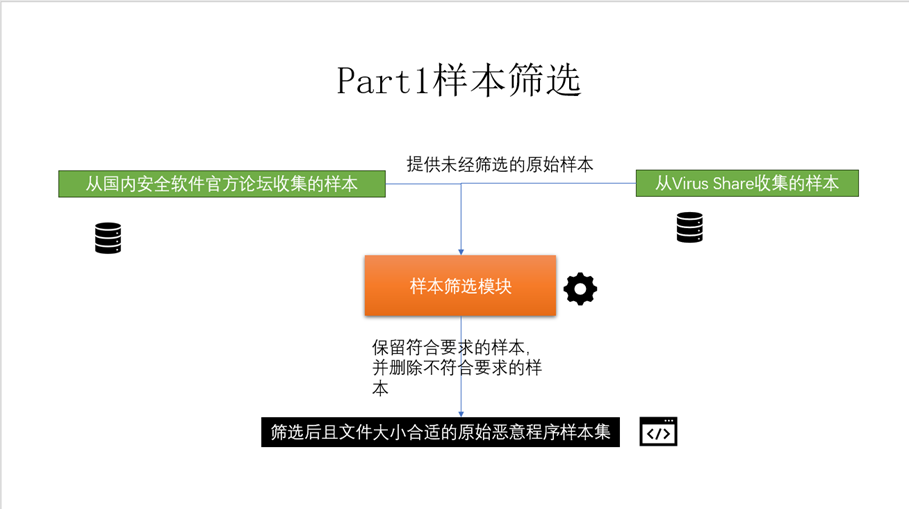
\includegraphics[]{images/system_design1.png}
  \caption{系统总体设计-1}\label{fig:system_design1}
\end{figure}

\begin{figure}
  \centering
  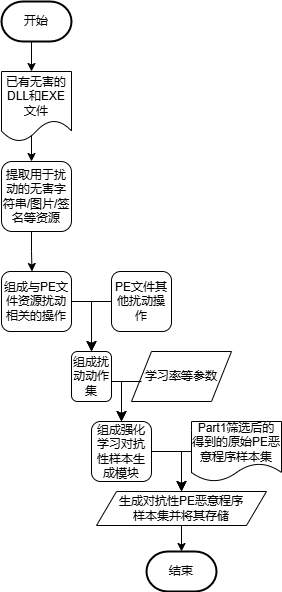
\includegraphics[]{images/system_design2.png}
  \caption{系统总体设计-2}\label{fig:system_design2}
\end{figure}

\begin{figure}
  \centering
  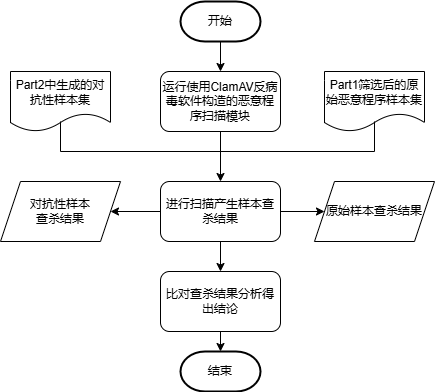
\includegraphics[]{images/system_design3.png}
  \caption{系统总体设计-3}\label{fig:system_design3}
\end{figure}

\section{样本筛选模块的设计与实现}

\subsection{设计思路}

\textcolor{black}{对于已收集到的样本(具体收集过程将在后文的实验中具体说明),需要注意的是,有些样本可能不是PE文件, 例如来源于火绒论坛上的一个样本包里面包含了恶意Windows Power Shell脚本和HTML恶意应用程序,恶意JavaScript脚本,恶意Visual Basic Script等非PE恶意程序。同时,因为本实验并没有对恶意动态链接库(DLL)和系统文件(SYS)进行对抗性样本生成,只是对恶意PE可执行文件(EXE)进行了对抗性样本生成,这是因为反病毒软件厂商提供的样本不包含动态链接库和系统文件,且检验动态链接库在对抗性样本生成后是否因为对抗性扰动导致损坏,相比检验PE可执行文件是否损坏更困难。所以,基于上述原因对于样本的筛选处理,理论上需要删除掉这些非PE可执行程序文件。}

\textcolor{black}{本实验设计样本筛选模块的原因是为了在实验中尽量避免有较大操作隐患的手动筛选,尽管手动筛选看起来很容易,但手动筛选很容易误操作,表现为用户可能意外执行恶意PE可执行程序导致可能遭受到恶意软件攻击。}

\textcolor{black}{筛选模块的输入应该是一个文件夹,其中包含待筛选的原始样本。对于来源于Virus Share的样本需要指定增加.exe后缀后的样本的输出位置,对于文件类型和大小的筛选可以直接使用Python的os模块删除不符合条件的样本文件,只保留实验需要用到的样本文件。 }

\textcolor{black}{每次处理的文件夹其中建议包含400~600个未筛选的恶意软件,收集好每次处理后的样本,并将这些样本归为一个样本集,为的是以备实验中后续使用。}

\textcolor{black}{然而,这种筛选方式在后续实验中可能会存在一些问题,具体将在后文中予以详细解释。}

\subsection{具体实现}

\textcolor{black}{样本筛选模块的具体实现思路如图\ref{fig:sample_swift_module}。图\ref{fig:sample_swift_module}是实现对于来源于Virus Share的样本进行筛选,对传入的绝对路径下的所有文件添加.exe文件扩展名,并且忽略传入的绝对路径下的文件夹,将添加扩展名后的样本与指定的输出路径拼接成输出文件名,之后进行拷贝操作,将原样本文件内容复制到新文件中,进而生成筛选后的样本。实现对于来源于国内安全软件论坛的样本筛选和VirusShare处理后的样本的二次筛选是通过对于传入的绝对路径,忽略路径下的文件夹,只考虑所有文件,会删除非PE可执行文件,即文件扩展名不为.exe的文件和大于4096字节大小的文件,最终保留下来的文件为符合条件的样本。}

\begin{figure}
  \centering
  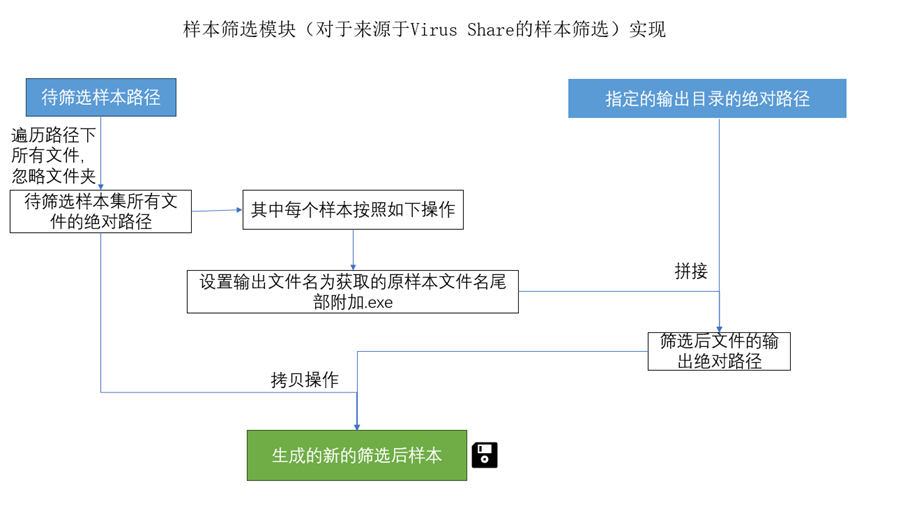
\includegraphics[]{images/sample_swift_module.png}
  \caption{样本筛选模块}\label{fig:sample_swift_module}
\end{figure}

\textcolor{black}{实验中的已设计好的样本筛选模块如图\ref{fig:configuration_of_sample_swift_module1},图\ref{fig:configuration_of_sample_swift_module2},图\ref{fig:configuration_of_sample_swift_module1}中对应的代码实现了对于来源于VirusShare的样本筛选,图\ref{fig:configuration_of_sample_swift_module2}中对应的代码实现了对于来源于VirusShare的样本二次筛选以及对于来源于国内安全软件论坛的样本筛选:}

\begin{figure}
  \centering
  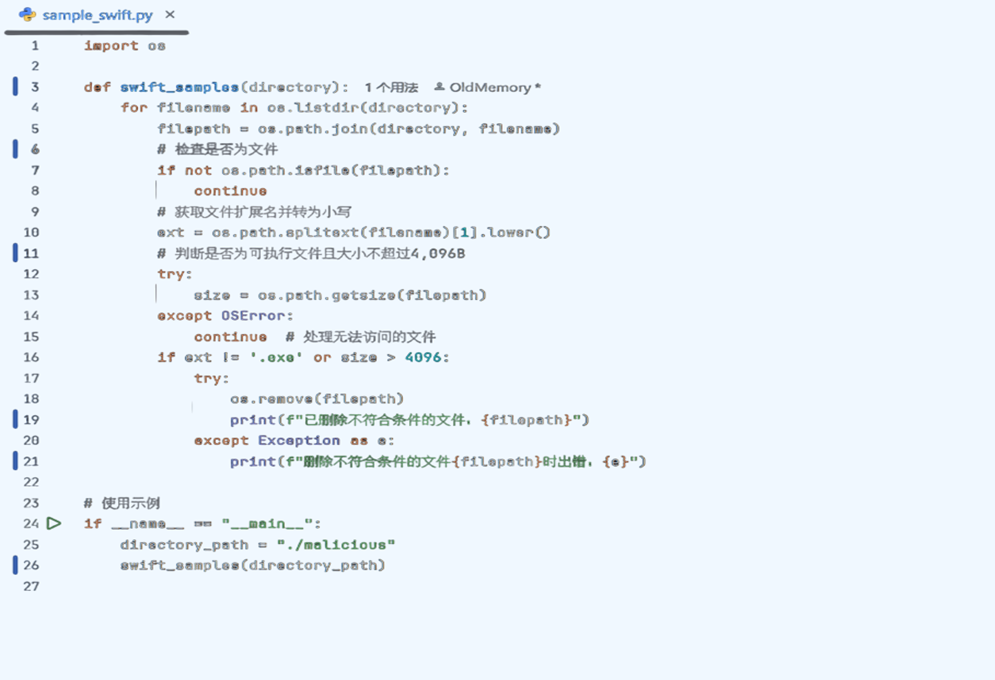
\includegraphics[]{images/configuration_of_sample_swift_module1.png}
  \caption{样本筛选模块配置1}\label{fig:configuration_of_sample_swift_module1}
\end{figure}

\begin{figure}
  \centering
  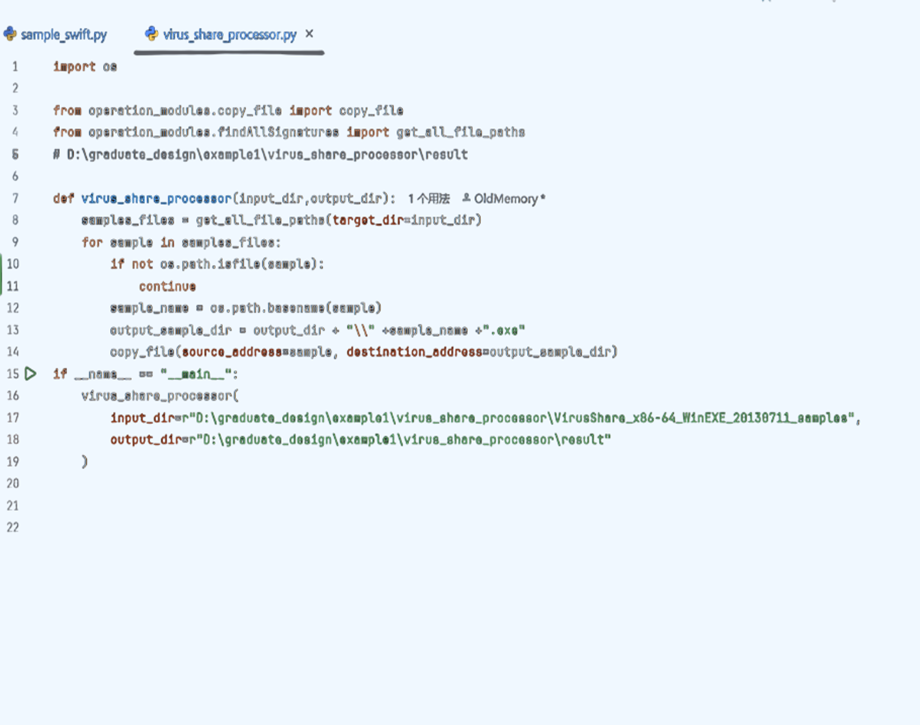
\includegraphics[]{images/configuration_of_sample_swift_module2.png}
  \caption{样本筛选模块配置2}\label{fig:configuration_of_sample_swift_module2}
\end{figure}

\textcolor{black}{为了考虑样本筛选模块的完备性,需要配备异常处理应对可能出现的一些异常情况:}

\textcolor{black}{(1)	传入的样本文件夹中包含子文件夹,筛选中需要忽略掉这些子文件夹。}

\textcolor{black}{(2)	传入的样本无法被访问,此时应该抛出异常警告。}

\section{恶意程序扫描模块设计与实现}

\subsection{设计思路}

\textcolor{black}{因为实验中需要判断样本的恶意性,所以需要搭建一个恶意软件检测器。在本实验中,选用了Python的pyclamed库的0.4.0版本搭建了一个基于ClamAV的恶意软件检测器。}

\textcolor{black}{恶意软件扫描模块的输入为待检测的PE可执行文件,输出结果为bool型,为true时,说明输入的PE可执行程序是恶意程序,为false时说明输入的PE可执行程序是良性程序。注意的是,检测器不应对输入的待检测的PE可执行文件做出任何修改。}

\textcolor{black}{然而,实验中恶意软件扫描模块可能会出现一些意想之外的情况,这将在后文会得到详细说明。}

\subsection{具体实现}

\textcolor{black}{恶意程序扫描模块的具体实现思路如图\ref{fig:malware_scan_module},需要传入待检测程序的绝对路径。图\ref{fig:malware_scan_module}对应的过程为:在模块运行前,用户通过命令手动更新本地ClamAV病毒库使其同步云端病毒库。模块运行时,主程序向主机的ClamAV服务发送TCP请求,如果这一步能成功,则ClamAV服务会查询其本地病毒库,如果这一步不成功,出现了TCP连接的超时问题,则会返回TCP连接错误,提示用户需要修复ClamAV服务。随后,ClamAV服务会依赖于本地病毒库对待检测程序进行扫描,再将扫描的结果通过TCP连接传递给主程序,主程序根据ClamAV服务的返回结果判断待检测程序是否是恶意软件。}

\begin{figure}
  \centering
  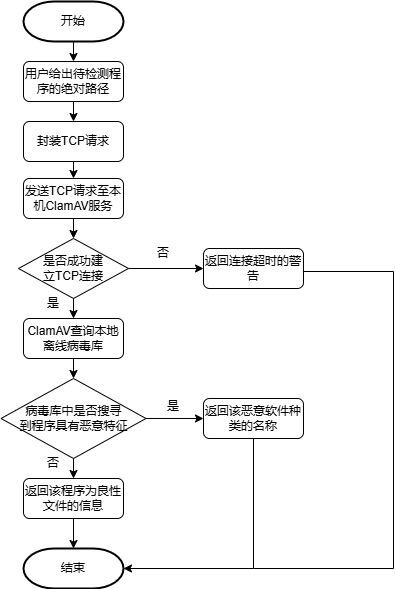
\includegraphics[]{images/malware_scan_module.png}
  \caption{恶意程序扫描模块}\label{fig:malware_scan_module}
\end{figure}

\textcolor{black}{为完成恶意程序扫描模块的视线,我们需要在主机配置ClamAV服务环境,首先需要在主机上安装ClamAV,并且修改安装目录下的clamd.conf文件,指定ClamAV服务的端口号。}

\textcolor{black}{为指定ClamAV服务的端口号,需要修改的是clamd.conf文件中TCP Socket的设置,因为是在本地配置ClamAV服务,clamd.conf中的TCPAddr,即TCP地址按照默认的localhost即可,无需修改。这一步需要注意端口号的冲突问题,最好事先检测主机已经使用的端口号,否则会影响恶意程序扫描模块的正常运行。}

\textcolor{black}{随后,需要修改freshclam.conf,这是因为ClamAV是基于本地病毒库来进行病毒扫描,需要配置病毒库地址和日志文件。}

\textcolor{black}{为了配置病毒库地址和日志文件,freshclam.conf中需要修改的项目是DataBaseDirectory和UpdateLogFile,分别对应ClamAV安装目录下的数据库目录和日志文件目录。}

\textcolor{black}{随后,打开cmd手动更新ClamAV病毒库,通过命令freshclam –config-file=./freshclam.conf实现对于ClamAV病毒库的更新操作,随后,ClamAV会从云端上下载病毒库。}

\textcolor{black}{更新数据库成功后。需要在Windows服务中重启ClamAV服务。这需要在服务的服务列表中选中ClamAV的ClamD服务左侧点击重启动该服务,或选中该服务右键,也可以达到重启该服务的目的。随后使用pyclamed库搭建恶意程序扫描模块,如图\ref{fig:configuration_of_malware_scan_module}所示,它的作用是检测传入的绝对路径指代的文件是否为恶意软件。需要输入待检测文件的绝对路径,随后会判断ClamAV服务是否处于活动状态,若不处于,则会抛出异常。随后执行文件扫描操作,判断文件是否为恶意软件,这是通过检测scanresult中的内容实现的。}

\begin{figure}
  \centering
  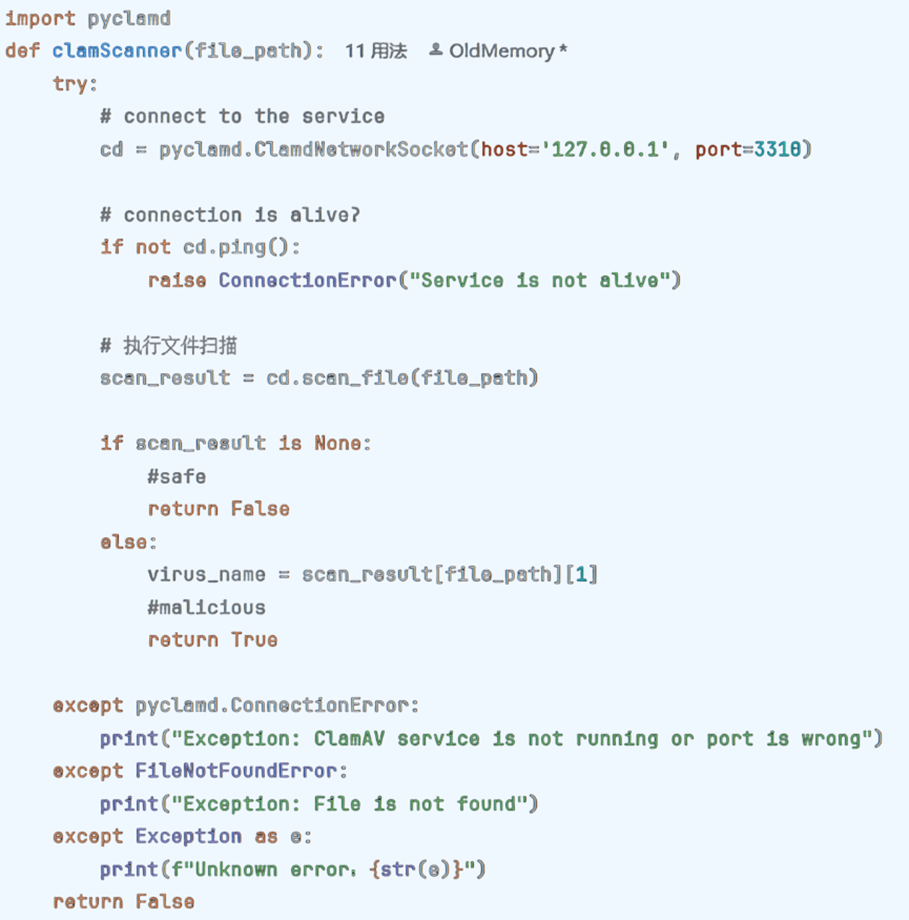
\includegraphics[]{images/configuration_of_malware_scan_module.png}
  \caption{恶意程序扫描模块配置}\label{fig:configuration_of_malware_scan_module}
\end{figure}

\textcolor{black}{模块功能需要考虑模块运行的完备性,在恶意软件扫描模块中需要处理一些可能存在的异常情况:}

\textcolor{black}{(1)需判断在特定端口号下运行的ClamAV服务是否处于活动状态,如果不处于活动状态,就抛出一个网络连接异常。如果没有考虑这个可能存在的异常,将会使样本检测结果不准确。这个问题多半发生于用户主机使用了网络代理软件,网络代理软件按照自身规则会将主机对于本机环回地址127.0.0.1下对于Clam AV服务端口的访问分配到其他主机,将会造成模块无法访问到主机ClamAV服务,进而无法正常工作。}

\textcolor{black}{(2)需要注意参数file\_path指定的绝对路径对应的文件是否存在,如果文件不存在,也需要抛出异常。当文件存在时,才允许调用scan\_file接口对该绝对路径下的文件进行扫描。}

\textcolor{black}{(3)具体实现中,ClamAV返回的扫描结果是字符串数组,为空说明传入的文件是良性文件,若传入的文件为恶意软件,则可在返回扫描结果中获取具体的恶意软件名称,但是具体的恶意软件名称对于本实验没有作用,不需要传回它们,只需要检测字符串数组是否为空即可判断文件是良性文件还是恶意软件。}

\section{强化学习对抗性样本生成模块设计与实现}

\subsection{设计思路}

\textcolor{black}{首先,我们需要设计强化学习模型可能对PE可执行程序修改采取的action,应包括如下内容:}

\textcolor{black}{(1)使用sigthief,将一个从良性软件中提取出的数字签名附加在恶意软件上,通过修改ImportTable中的CertTableLOC,CertLOC,CertSize等内容实现,操作后的结果如图\ref{fig:certification_fabrication}所示,可以发现恶意程序被附加了一个可信任的CA证书,该证书由Xing Wang发行,从Xilinx的软件安装包上剥落而来。}

\begin{figure}
  \centering
  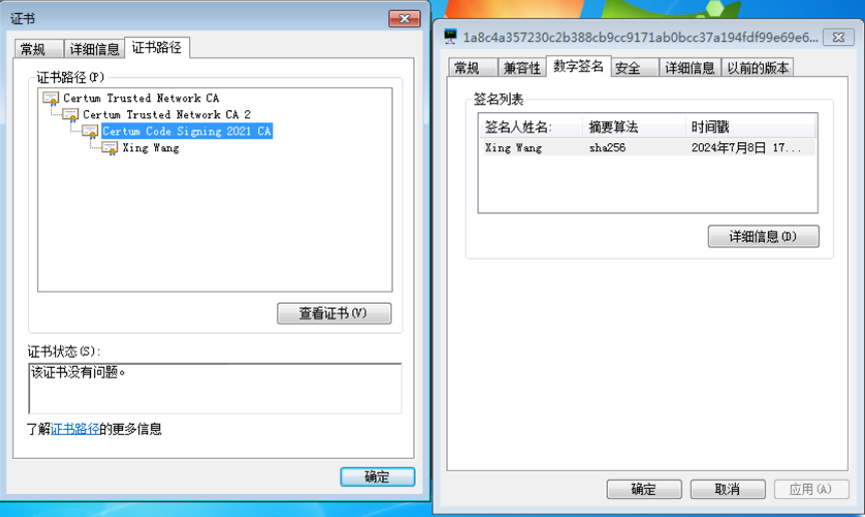
\includegraphics[]{images/certification_fabrication.png}
  \caption{恶意程序扫描模块配置}\label{fig:certification_fabrication}
\end{figure}

\textcolor{black}{(2)在PE程序的尾部添加无意义的字节:}

\textcolor{black}{添加的字节使用随机生成的字符串或一些良性动态链接库的.text段。}

\textcolor{black}{(3)修改校验和(checksum):}

\textcolor{black}{需要指定修改后的checksum内容,将可选首部的Checksum字段修改为指定后的内容}

\textcolor{black}{(4)修改机器码:}

\textcolor{black}{修改PE可执行文件的Machine和Magic内容。但如果一旦修改后的机器码和软件运行平台的机器码不同,则程序会无法启动。然而,这会引起恶意软件损坏的问题,在后续被弃用。}

\textcolor{black}{(5)修改时间戳:}

\textcolor{black}{此功能本实验用pefile库和lief库分别实现了该功能,函数会随机生成一个过去一年之内的时间对应的时间戳,并且将生成的时间戳替换掉恶意软件原有的时间戳。}

\textcolor{black}{(6)UPX加壳操作:}

\textcolor{black}{使用The Ultimate Packer for executables加壳工具,是GitHub网站上的一个开源壳项目。读者可以访问https://github.com/upx/upx获取加壳工具。}

\textcolor{black}{同时,它也能做到压缩原PE可执行程序的大小。}

\textcolor{black}{在运行UPX加壳操作时需要注意UPX加壳程序的路径,防止因为路径问题导致抛出异常加壳失败。}

\textcolor{black}{(7)向节之间的空洞中添加无意义的字节:}

\textcolor{black}{添加的字节使用随机生成的字符串或一些良性动态链接库的.text段。}

\textcolor{black}{同时,也需要一个search\_cave()函数用于寻找节之间的空洞。}

\textcolor{black}{(8)修改导入表,增加PE可执行程序导入的函数:}

\textcolor{black}{从small\_dll\_imports.json中选取导入的函数来修改导入表,会添加引用的动态链接库或函数。}

\textcolor{black}{(9)在PE可执行文件后添加一个节,节中包含无意义的字符串数据:}

\textcolor{black}{此操作使用LIEF库实现,添加的字节使用随机生成的字符串或一些良性动态链接库的.text段。}

\textcolor{black}{(10)修改PE可执行程序首部校验和:}

\textcolor{black}{将PE可执行程序的首部校验和修改成0。}

\textcolor{black}{(11)删除PE可执行程序的调试信息:}

\textcolor{black}{可能因为没有debug信息,导致操作无意义,但不会抛出异常。}

\textcolor{black}{(12)重命名原PE可执行程序中的某个节,备选的重命名名称会在
.abitcsa .bbitcsb .cbitcsc .dbitcsd .ebitcse .fbitscf .gbitcsg .hbitcsh .ibitcsi .jbitcsj .kbitcsk中随机选择一个。
}

\textcolor{black}{(13)向原PE可执行程序中增加资源:}

\textcolor{black}{增加的资源是多个ICO文件,是从备选的ICO文件中随机选取,然后截取随机大小,再调用resourcehacker将处理后的ICO文件加入到资源中。}

\textcolor{black}{这些action的传入参数应包含待修改的可执行文件,经过对抗性操作修改后生成对抗性样本,随后,这些对抗性样本需要被移动到原路径以完成修改。}

\textcolor{black}{对于对抗性样本生成的强化学习算法设计如下,其包含三个算法模块,主算法实现对抗性样本生成的功能,子算法2和子算法3实现训练,总奖励更新的功能。主算法用于强化学习对抗性样本生成模块运行。}

\textcolor{black}{主算法:}

\textcolor{black}{功能:对抗性样本生成函数}

\textcolor{black}{输入: 样本集目录sample\_directory,强化学习模型Sarsa\_model }

\textcolor{black}{输出: 生成的对抗性样本}

\textcolor{black}{算法伪代码:}

\begin{lstlisting}[language=Python, caption={code for main alogrithm}, label={lst:pythonfile1}]
def alogrithm_generate_controversy_samples(sample_directory,actions_list,Sarsa_model):  
	Sarsa_model.init(actions_list,gamma,alpha,epsilon) #init
	evasion_count = train(Sarsa_model,sample_directory)
\end{lstlisting}

\textcolor{black}{主算法实现了对于强化学习模型的初始化和样本训练结束后统计成功逃逸的样本数量}

\textcolor{black}{子算法1:}

\textcolor{black}{功能:完成主算法中的训练操作(train)}

\textcolor{black}{输入:样本集目录sample\_directory,强化学习模型Sarsa\_model}

\textcolor{black}{输出:成功逃逸的对抗性样本数量}

\textcolor{black}{算法伪代码:}

\begin{lstlisting}[language=Python, caption={code for sub alogrithm 1}, label={lst:pythonfile2}]
def train(Sarsa_model,sample_directory):  
    episodes = get_episodes_for_training(sample_directory)   #get samples
    evasion_count = 0   
    for episode in episodes:  
        count = 0   #init
        state = 0  
        total_reward = 0   
        status_done = False   
        reward = 0   
        action = choose_action(state)   #choose action
        do_action(action,episode)   
        while not status_done:
      #total reward update
      total_reward=update_total_reward(episode,total_reward)
            if status_done: #not final state
                Sarsa_model.update(state,action,reward,next_state=None,next_action=None)   
            else:   # final state
                next_action = choose_action(next_state)   
                Sarsa_model.update(state,action,reward,next_state,next_action)   
                action = next_action   
                do_action(action,state,enable_log)   
    return evasion_count
\end{lstlisting}

\textcolor{black}{子算法1实现了对于样本集中的每个样本,根据当前状态在行为表中选择操作并且执行,若当前状态为终止态,则更新强化学习模型并对下一个样本进行操作,否则继续选择操作并且予以执行。}

\textcolor{black}{子算法2:}

\textcolor{black}{功能:完成子算法1中的对total\_reward的更新操作}

\textcolor{black}{输入: 当前的样本episode,更新前的总奖励total\_reward}

\textcolor{black}{输出: 更新后的总奖励total\_reward}

\textcolor{black}{算法伪代码:}

\begin{lstlisting}[language=Python, caption={code for sub alogrithm 2}, label={lst:pythonfile3}]
def update_total_reward(episode,total_reward):  
    judgement = can_evasion(episode)   
        if judgement == True :    # can evade detect
            evasion_count++   
            next_state = None  # reach final state
            reward = SUCCESS_REWARD   
            status_done = True   
        else:  
            count++   
            if count >= Max_Count:  # operations amount run out
                reward = FAIL_REWARD   
                next_state = None   
                status_done = True   # reach final state
            else:  # operations amount do not run out
                next_state = count   
    total_reward+=reward   # update total reward
    return total_reward  
\end{lstlisting}

\textcolor{black}{子算法2实现了对于总奖励和状态的更新,当能成功逃逸恶意软件扫描模块的检测时,进入终止态并且获得奖励,若不能逃逸,进行判断,如果次数已经达到最大次数,则进入终止态并且获取奖励,否则更新状态。最后返回总奖励。}

\textcolor{black}{强化学习算法的总工作流程如下描述:}

\textcolor{black}{Step1:传入恶意样本集的目录和其它参数,先将恶意样本的绝对目录存储,以备后续Sarsa智能体模型使用,同时预加载Sarsa模型(Sarsa\_model)。}

\textcolor{black}{Step2:对于样本集中的每个样本episode,先初始化奖励。}

\textcolor{black}{Step3:根据状态当前选择一个行为,episode经由处理后,经由前文中封装的恶意程序扫描模块,检测是否成功逃逸反病毒软件的扫描。}

\textcolor{black}{Step4:如果成功,则直接进入终止态,获取奖励SUCCESS\_REWARD并且更新Sarsa模型的Qtable,否则进入下一个状态}

\textcolor{black}{Step5:如果失败,但是次数没有达到Max\_Count,则更新Sarsa模型的Qtable,并且重复Step3的过程。如果失败且次数达到了Max\_Count,进入终止状态,并获取奖励FAIL\_REWARD(可以设置为负数,也可以设置为0)和更新Sarsa模型的Qtable。}

\textcolor{black}{这个算法在后续实验中也允许被略微修改,用于实现对强化学习模型采取某些行为的鼓励,例如可以修改为执行添加新的节的行为在完成后会有较小的奖励以鼓励智能体更多执行该行为。}

\subsection{具体实现}

\textcolor{black}{行为表中的部分action的具体实现思路如图\ref{fig:peel_signature},图\ref{fig:append_signature},图\ref{fig:get_benign_strings},图\ref{fig:append_strings},图\ref{fig:modify_checksum},图\ref{fig:modify_timestamp},图\ref{fig:append_benign_sections},图\ref{fig:add_resources}所示。}

\textcolor{black}{图\ref{fig:peel_signature}描述了SigThief获取良性程序签名的过程,需要预备一些良性应用程序,首先SigTheif会检测与数字签名相关的ImportTable中的CertTableLoc,CertSize条目,如果不存在,则SigThief认为该良性文件不能获取到签名,直接跳过改文件,如果存在,则在CertLoc位置截取CertSize大小的字符,即为数字签名对应的字符串,并将其保存至一个.exe\_sig扩展名的文件,作为从良性文件上剥落的签名,以备后续为恶意软件添加数字签名。}

\textcolor{black}{图\ref{fig:append_signature}描述了SigThief将从良性文件上剥落的签名(格式为.exe\_sig)附加在恶意软件上的过程,需要前一步生成的.exe\_sig文件作为签名内容,具体过程为修改输入的恶意软件中的CertTableLoc等内容,并将输入中剥落下的良性签名的内容追加在恶意软件末尾,随后将修改后的恶意软件输出至指定的绝对路径下。}

\textcolor{black}{图\ref{fig:get_benign_strings}描述了良性字符串的获取过程,需要预备一些良性文件(可以是PE可执行程序、动态链接库、系统文件),此过程首先会判断良性文件的内容,如果不含.text节(实际上也可以指定为.data节或其他节),则直接跳过该良性文件,如果含有,则将.text节中全部内容保存在一个字符串中,以备后续过程使用。}

\textcolor{black}{图\ref{fig:append_strings}描述了恶意软件尾部追加无意义字节的具体过程,首先会将待处理的恶意程序读取为二进制字符串,随后从获取到的良性字符串中随机选取一个,使用字符串拼接操作加在待处理的恶意程序二进制字符串尾部,最后,将拼接后的二进制字符串写入指定的目录下完成对恶意软件进行无意义字节的追加操作。}

\textcolor{black}{图\ref{fig:modify_checksum}描述了恶意软件修改校验和的具体过程,首先会将待处理的恶意程序读取为二进制字符串,随后会修改可选首部的CheckSum字段为目标校验和,最后,将修改后的二进制字符串写入指定的目录下完成对恶意软件进行修改校验和的操作。}

\textcolor{black}{图\ref{fig:modify_timestamp}描述了恶意软件修改时间戳的具体过程,首先会将待处理的恶意程序读取为二进制字符串,随后会修改首部的TimeDateStamp字段为目标校验和,最后,将修改后的二进制字符串写入指定的目录下完成对恶意软件进行修改时间戳的操作。}

\textcolor{black}{图\ref{fig:append_benign_sections}描述了恶意软件尾部增加无意义资源节的具体过程,最开始完成的操作是决定新增加节的名称,需要获取恶意软件中所有节的名称,并且与所有预先设定好的备选节名称做差集,得到的结果为可用的备选节名称,在其中随机选取一个座位新增加的节的名称。新增加的节中的内容可从良性字符串集合中任选一个。在选取新增节的名称和新增节的内容后,使用lief库的add\_section操作即可对恶意软件进行新增节的操作。}

\textcolor{black}{图\ref{fig:add_resources}描述了恶意软件添加新的图标资源的具体过程,首先需要预备一些带有图标的良性文件集合,使用resourcehacker从中提取ico图标资源。在操作进行前,需要对提取到的ico图标资源进行修改像素和截取操作生成待添加的备用图标资源,确保每次添加的图标资源都不同。最后,通过cmd调用resourcehack完成对恶意软件新增图标资源的操作,指定操作为addskip,待添加资源res为生成的备用图标资源中随机选取的一个备用资源图标。}

\begin{figure}
  \centering
  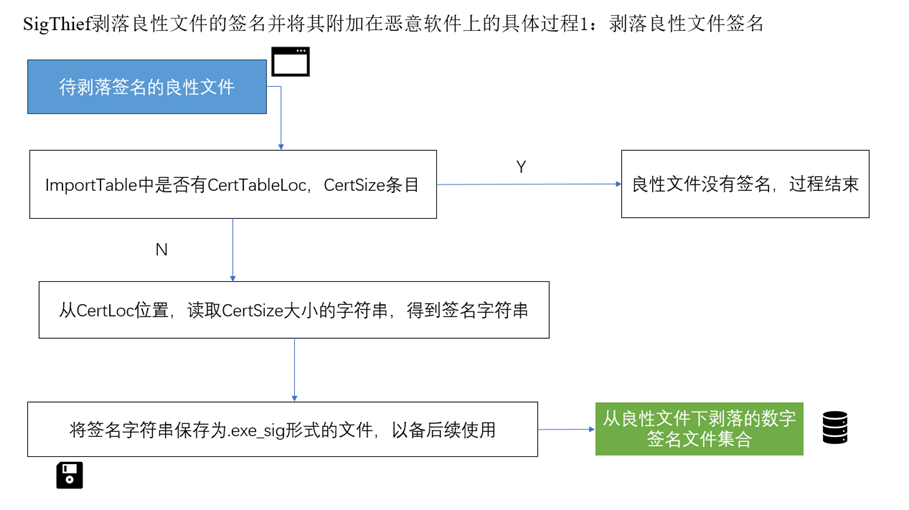
\includegraphics[]{images/peel_signature.png}
  \caption{剥落签名}\label{fig:peel_signature}
\end{figure}

\begin{figure}
  \centering
  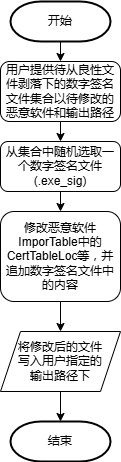
\includegraphics[]{images/append_signature.png}
  \caption{附加签名}\label{fig:append_signature}
\end{figure}

\begin{figure}
  \centering
  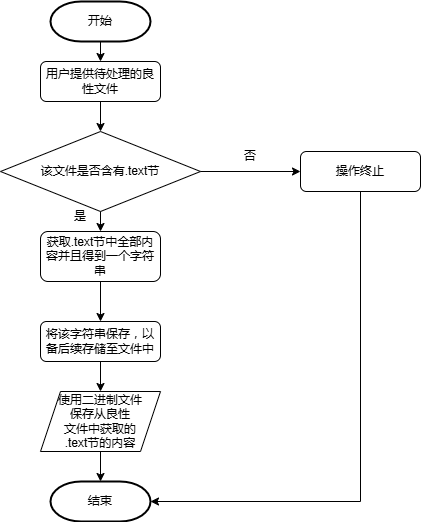
\includegraphics[]{images/get_benign_strings.png}
  \caption{获取良性字符串}\label{fig:get_benign_strings}
\end{figure}

\begin{figure}
  \centering
  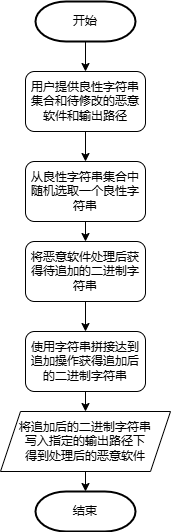
\includegraphics[]{images/append_strings.png}
  \caption{尾部追加无意义字节}\label{fig:append_strings}
\end{figure}

\begin{figure}
  \centering
  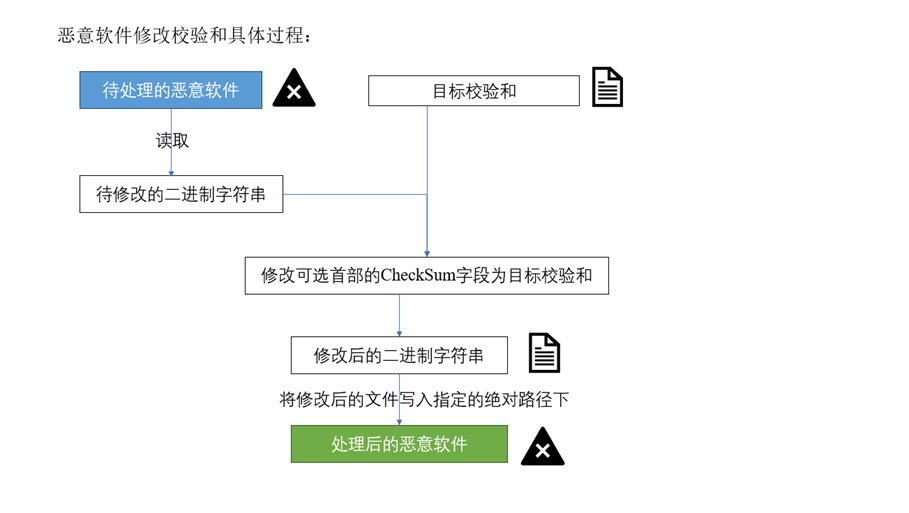
\includegraphics[]{images/modify_checksum.png}
  \caption{修改校验和}\label{fig:modify_checksum}
\end{figure}

\begin{figure}
  \centering
  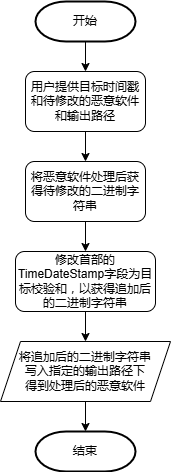
\includegraphics[]{images/modify_timestamp.png}
  \caption{修改时间戳}\label{fig:modify_timestamp}
\end{figure}

\begin{figure}
  \centering
  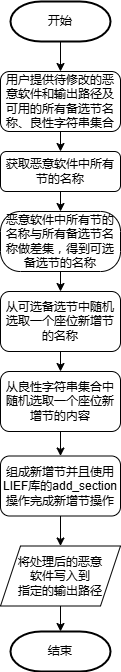
\includegraphics[]{images/append_benign_sections.png}
  \caption{尾部追加无意义资源节}\label{fig:append_benign_sections}
\end{figure}

\begin{figure}
  \centering
  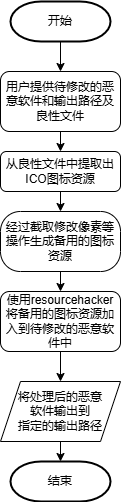
\includegraphics[]{images/add_resources.png}
  \caption{添加新的图标资源}\label{fig:add_resources}
\end{figure}

\textcolor{black}{图\ref{fig:reinforcement_learning_adversarial_sample_generation_module}中描述了强化学习对抗性样本生成模块的具体工作过程,对于传入样本集中的每个样本,首先设定最初奖励为0、总奖励为0、已进行操作数量为0、终态为否,再根据状态选择其执行的行为,在每次执行行为结束后,检测其是否能逃逸ClamAV的查杀,若能成功逃逸ClamAV查杀,则获取奖励后,进入终止态,并更新强化学习模型的Qtable和更新成功逃逸数量,随后处理下一个样本;若不能成功逃逸ClamAV查杀,则操作次数+1,此时再判断操作数量是否已经达到最大数量,如果已经达到了最大数量,则进入终止态,并且获取相应惩罚,并更新强化学习模型的Qtable,随后将处理下一个样本;如果没有达到最大数量,则更新强化学习模型的Qtable后,进入一个新的状态,并重复上述操作,直到传入样本集中的所有样本都被处理完为止,处理结束后,最终返回处理后能成功逃逸ClamAV查杀的样本数。同时为了提高图\ref{fig:reinforcement_learning_adversarial_sample_generation_module}中设计的强化学习对抗性样本生成模块的健壮性,我们需要考虑修正强化学习对抗性样本生成模块需要用到的行为表,先前强化学习对抗性样本生成模块关于行为表的设计是合理的,但缺乏健壮性,可能会存在一些隐患,导致某些行为被执行时可能会抛出异常进而导致整个程序崩溃。}

\begin{figure}
  \centering
  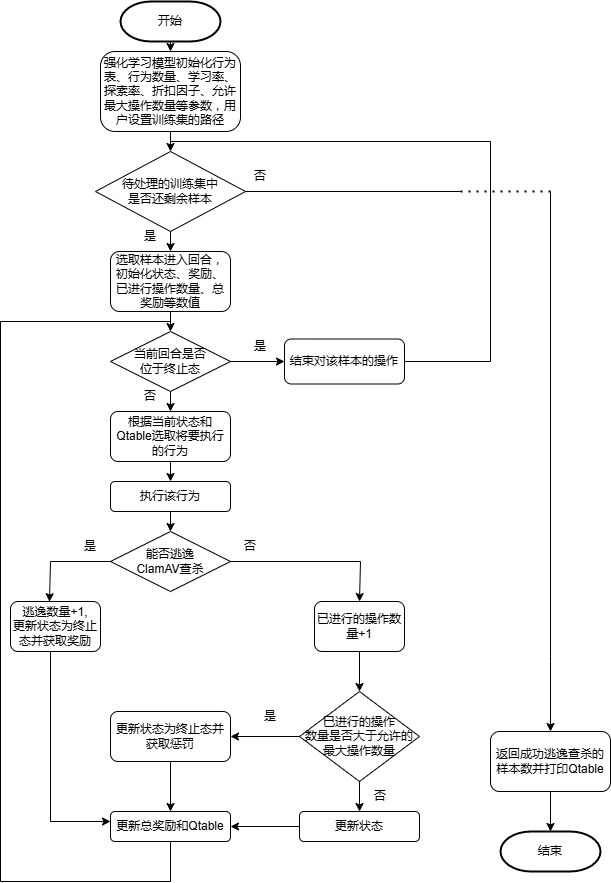
\includegraphics[]{images/reinforcement_learning_adversarial_sample_generation_module.png}
  \caption{强化学习对抗性样本生成模块}\label{fig:reinforcement_learning_adversarial_sample_generation_module}
\end{figure}

\textcolor{black}{原因如下:}

\textcolor{black}{(1)样本筛选无法删掉一些伪装的PE可执行文件,尽管这些文件后缀名是.exe,但这些文件使用了结构化欺骗,实际上这些文件自身并不含有COFF文件头等内容,例如一个原本后缀是.sys的程序,后缀被篡改为.exe,如果action在执行时认为它们是PE可执行文件并且对其操作,就会因为PE格式解析异常报错,进而Python主程序将会抛出异常,没有被处理的异常会导致整个程序被迫终止。解决方案是通过为do\_action()函数设置异常处理的代码块来解决这个问题,即使遇到了不是正常的PE可执行文件,程序仍然因为不会抛出异常,导致强制终止整个程序。}

\textcolor{black}{(2)存在一些PE可执行文件恶意软件,自身大小非常大,大约64MB到数百MB,可能是这些文件本身已经经过了一些对抗性操作导致的,笔者在测试中发现,对抗性操作在处理它们时极其缓慢,有些甚至需要数分钟的时间,这无疑严重拖累了对抗性处理操作执行的速度。其次,这些较大的PE可执行程序读取和写入操作对磁盘的损害也是巨大的,极有可能在运行中发生系统蓝屏死机的问题,甚至可能会导致数据丢失。解决方案在样本筛选模块已提出,即样本中大于4096字节的PE可执行程序在筛选样本时需要被删除,以避免后续操作出现故障导致程序强制终止。}

\textcolor{black}{(3)对于(1)中的问题,在异常处理的基础上,应该额外为action配备日志系统来监控对于PE可执行文件的修改操作。同时记录修改前和修改后文件的SHA256哈希值和使用的操作名称在一个日志文件中。配备日志系统有利于进行对于单个action的黑盒测试时排查错误,以及根据文件的哈希值判断这些对抗性干扰操作是否有效。修改成功的一个必要条件是修改后文件的哈希值与修改前文件的哈希值不同。如图\ref{fig:log_module}所示,图\ref{fig:log_module}中表明是为PE文件尾部添加冗余良性字节的操作配备日志,其中使用了logging.basicConfig相关设定来指定日志格式,同时,日志系统最好设置为允许开关,否则可能会在使用较差的硬盘时导致IO时间浪费在日志输出上。}

\textcolor{black}{(4)部分action可能会造成原有恶意程序被破坏,例如修改机器码操作,实际测试证明它会损坏恶意程序,所以在操作集中不应该包含它。}

\textcolor{black}{(5)部分action如UPX加壳,调用resource hacker加资源,sigthief仿造签名等操作,是通过cmd调用已有应用程序实现,可能会存在进程同步异步问题,可以利用Python自身time库的sleep函数来解决。}

\begin{figure}
  \centering
  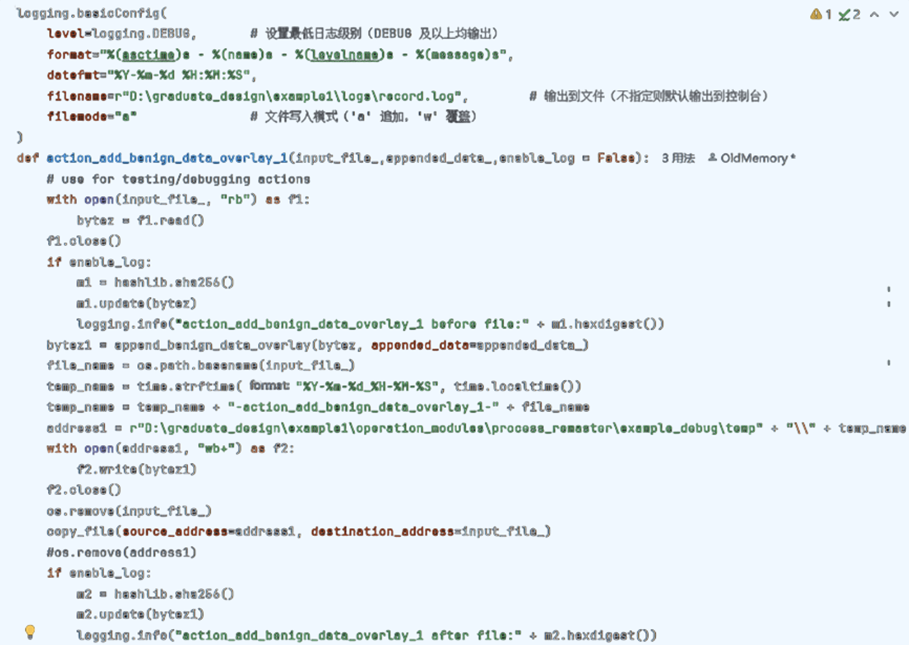
\includegraphics[]{images/log_module.png}
  \caption{日志系统}\label{fig:log_module}
\end{figure}

\textcolor{black}{随后,如图\ref{fig:init_pramameter}所示,在运行前,需要调整Sarsa算法的初始参数中的学习率alpha,探索率gamma,折扣因子epsilon。}

\begin{figure}
  \centering
  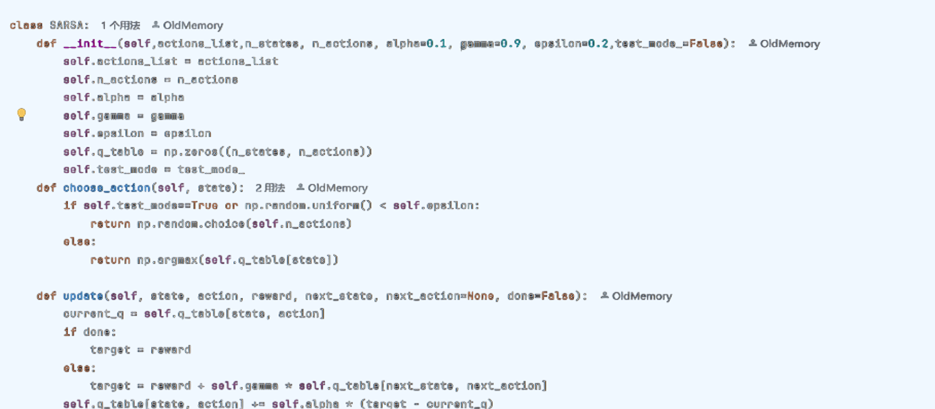
\includegraphics[]{images/init_pramameter.png}
  \caption{日志系统}\label{fig:init_pramameter}
\end{figure}

\textcolor{black}{本实验在强化学习对抗性样本生成模块中实际构建中额外引入了惩罚因子,它与恶意PE可执行文件处理前后的大小有一定关系,式3-1定义了文件大小改变比:}
\begin{equation}
    k=size_{after}/size_{before}
\end{equation}

\textcolor{black}{式3-2定义惩罚因子$\sigma_{1}$:}
\begin{equation}
    \sigma_{1}=1/((1/3)*lnk+1)
\end{equation}

\textcolor{black}{因此,成功达到最终状态获取的奖励$reward$会被再次修正为$reward=reward*\sigma_{1}$。}

\textcolor{black}{看似能尽量促进智能体选择尽量不过分扩大原恶意PE可执行文件的大小,然而实行运行时很小概率下会发生问题,这表现在使用UPX加壳后,$size_{after}$过于小,导致惩罚因子$\sigma_{1}$变成负数,理论上本该因为达成了逃逸效果,被Clam AV检测为良性程序,应该获取的是正数的奖励,但实际上获取的是负值奖励,这与达成逃逸获取正数奖励的设定矛盾。}

\textcolor{black}{因此,最好修正惩罚因子,修正后的惩罚因子在式3-3中定义为$\sigma_{2}$。}
\begin{equation}
    \sigma_2=(1/k)^2
\end{equation}

\textcolor{black}{这样可以避免使惩罚因子变为负数,从而影响智能体做出更优的决策的意外。}

\section{本章小结}

\textcolor{black}{本章首先介绍了实现强化学习的静态对抗性样本生成系统的设计与实现,将其分为三个模块,并描述需要各个模块的大致设计和需要实现的功能,介绍了对抗性样本生成的算法,恶意程序扫描模块,恶意程序样本筛选的方法。}